\documentclass[10pt,a4paper]{article}
\usepackage[utf8]{inputenc}
\usepackage[T1]{fontenc}
\usepackage{lmodern}
% Español si el paquete está instalado (Overleaf/MiKTeX lo traen); si no, nombres a mano
\IfFileExists{spanish.ldf}{%
  \usepackage[spanish,es-noshorthands,es-tabla]{babel}%
}{%
  \AtBeginDocument{\renewcommand{\figurename}{Figura}\renewcommand{\tablename}{Tabla}}%
}
\usepackage[a4paper,margin=1.9cm,top=1.7cm,bottom=1.8cm]{geometry}
\usepackage{microtype}
\usepackage{xcolor}
\usepackage{amsmath}
\usepackage{booktabs,tabularx,multirow}
\usepackage{listings}
\usepackage{tikz}
\usetikzlibrary{positioning,arrows.meta,calc,fit,backgrounds,decorations.pathreplacing}
\usepackage{enumitem}
\usepackage[font=small,labelfont=bf,skip=3pt]{caption}
\usepackage{fancyhdr}
\usepackage[colorlinks=true,linkcolor=azul,urlcolor=azul,citecolor=azul]{hyperref}

\definecolor{azul}{HTML}{1F4E79}
\definecolor{gris}{HTML}{F3F4F6}
\definecolor{grisT}{HTML}{6B7280}
\definecolor{verde}{HTML}{2E7D32}
\definecolor{rojo}{HTML}{B3261E}
\definecolor{naranja}{HTML}{C2620A}
\definecolor{cHdr}{HTML}{DCE6F2}
\definecolor{cSub}{HTML}{E8F1E4}
\definecolor{cArt}{HTML}{FFF1D6}

\setlength{\parindent}{0pt}
\setlength{\parskip}{3.5pt}
\setlist{nosep,leftmargin=*}

\pagestyle{fancy}
\fancyhf{}
\renewcommand{\headrulewidth}{0.3pt}
\fancyhead[L]{\small\color{grisT}RCI · Visualizador de un UR3e por TCP/IP}
\fancyhead[R]{\small\color{grisT}Memoria breve}
\fancyfoot[C]{\small\thepage}

\lstdefinestyle{py}{
  language=Python, basicstyle=\ttfamily\footnotesize, keywordstyle=\color{azul}\bfseries,
  commentstyle=\color{verde}\itshape, stringstyle=\color{naranja}, backgroundcolor=\color{gris},
  frame=leftline, rulecolor=\color{azul}, framerule=1.5pt, xleftmargin=16pt, framexleftmargin=13pt,
  numbers=left, numberstyle=\tiny\color{grisT}, numbersep=6pt, showstringspaces=false,
  breaklines=true, columns=fullflexible, keepspaces=true, aboveskip=4pt, belowskip=2pt,
  literate={á}{{\'a}}1 {é}{{\'e}}1 {í}{{\'i}}1 {ó}{{\'o}}1 {ú}{{\'u}}1 {ñ}{{\~n}}1 {±}{{$\pm$}}1
}
\lstset{style=py}
\newcommand{\code}[1]{\texttt{\small #1}}
\newcommand{\preg}[2]{\par\smallskip\noindent{\color{azul}\bfseries P#1.}~{\itshape #2}\par\nopagebreak}

\begin{document}

%======================== PORTADA COMPACTA ========================
\begin{center}
{\LARGE\bfseries\color{azul} Visualizador de un UR3e por TCP/IP}\\[3pt]
{\large Práctica guiada · Redes de Comunicación Industriales (MUAECI)}\\[3pt]
{\normalsize Angel Ardila · Universidad de Deusto · Octubre de 2026}\\[2pt]
{\small Repositorio: \url{https://github.com/angeloob11/TCP_ER_SERVER}}
\end{center}
\vspace{-4pt}
\noindent\rule{\linewidth}{0.4pt}

\section{Estructura del código}

El programa es un cliente TCP escrito en Python 3.12 que lee el estado de uno o varios UR3e (URSim o robot real), lo dibuja en PyBullet con el paquete \code{UR3e\_rg2} y, en el nivel de sobresaliente, envía programas URScript. Todo el código de comunicación es propio y está repartido en seis módulos (tabla~\ref{tab:modulos}). La decodificación de cada interfaz vive en un solo sitio y la reutilizan tanto los scripts de un robot como \code{multi\_robot.py}.

\begin{table}[h]
\centering\small
\caption{Módulos de \code{src/} y su responsabilidad.}\label{tab:modulos}
\begin{tabularx}{\linewidth}{@{}l r X@{}}
\toprule
Módulo & Líneas & Responsabilidad \\ \midrule
\code{buffer\_ur.py} & 45 & Conexión con reintento y \emph{timeout}; buffer \code{bytearray} y troceo del flujo por longitud. Lo usan las dos interfaces. \\
\code{primaria.py} & 98 & Lector del puerto 30001: tipo 16 (subpaquetes 0 y 1) y tipo 20 (errores). Visualizador de un robot. \\
\code{tiempo\_real.py} & 99 & Lector del puerto 30003 por desplazamientos fijos, con medida de paquetes/s. Visualizador de un robot. \\
\code{multi\_robot.py} & 477 & Varios robots desde \code{config/robots.json}, un hilo y un \code{Lock} por robot, enseñar y reproducir. \\
\code{rx.py} & 107 & Diagnóstico sin hilos: compara el reloj del robot con el del PC para medir la tasa real. \\
\code{constantes.py} & 5 & IP y puertos por defecto, $v_{\max}=0{,}3$\,rad/s y $a_{\max}=0{,}5$\,rad/s$^2$. \\ \bottomrule
\end{tabularx}
\end{table}

\vspace{-6pt}
La arquitectura (figura~\ref{fig:arq}) separa la \textbf{recepción}, con un hilo lector por robot que consume todo lo que llega y guarda solo el último estado, del \textbf{dibujo}, un bucle principal a 30\,Hz que copia ese estado y mueve el robot de PyBullet. Así la interfaz de 500\,Hz no acumula retraso por culpa del renderizado. Las órdenes URScript se envían por el mismo socket que usa el lector: como ese hilo nunca deja de leer, el buffer de recepción del sistema operativo no se llena y la conexión no se bloquea.

\begin{figure}[h]
\centering
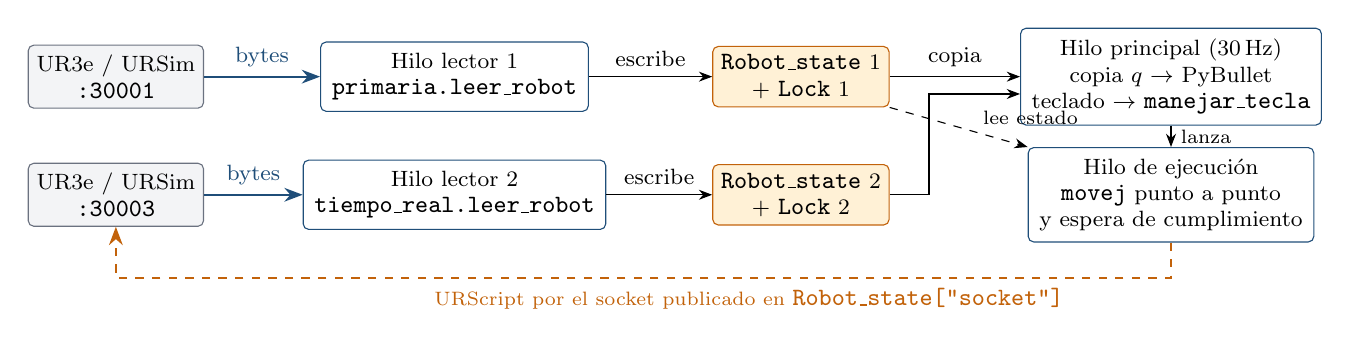
\begin{tikzpicture}[font=\footnotesize, >=Stealth,
  caja/.style={draw=azul, rounded corners=2pt, fill=white, align=center, inner sep=4pt, minimum height=8mm},
  robot/.style={draw=grisT, rounded corners=2pt, fill=gris, align=center, inner sep=3pt, minimum width=17mm, minimum height=8mm},
  dato/.style={draw=naranja, fill=cArt, rounded corners=2pt, align=center, inner sep=3pt}]
\node[robot] (r1) at (0,0.6) {UR3e / URSim\\ \code{:30001}};
\node[robot] (r2) at (0,-0.9) {UR3e / URSim\\ \code{:30003}};
\node[caja, minimum width=34mm] (l1) at (4.3,0.6) {Hilo lector 1\\\code{primaria.leer\_robot}};
\node[caja, minimum width=34mm] (l2) at (4.3,-0.9) {Hilo lector 2\\\code{tiempo\_real.leer\_robot}};
\node[dato] (s1) at (8.7,0.6) {\code{Robot\_state} 1\\ + \code{Lock} 1};
\node[dato] (s2) at (8.7,-0.9) {\code{Robot\_state} 2\\ + \code{Lock} 2};
\node[caja, minimum width=33mm] (main) at (13.4,0.6) {Hilo principal (30\,Hz)\\copia $q$ $\rightarrow$ PyBullet\\teclado $\rightarrow$ \code{manejar\_tecla}};
\node[caja, minimum width=33mm] (ej) at (13.4,-0.9) {Hilo de ejecución\\\code{movej} punto a punto\\y espera de cumplimiento};
\draw[->, thick, azul] (r1) -- node[above]{bytes} (l1);
\draw[->, thick, azul] (r2) -- node[above]{bytes} (l2);
\draw[->] (l1) -- node[above]{escribe} (s1);
\draw[->] (l2) -- node[above]{escribe} (s2);
\draw[->] (s1) -- node[above]{copia} (main);
\draw[->] (s2.east) -- ++(0.5,0) |- ($(main.west)+(0,-0.22)$);
\draw[->, dashed] (s1.south east) -- node[pos=0.62,above right=-1pt]{\scriptsize lee estado} (ej.north west);
\draw[->, dashed, naranja, thick] (ej.south) -- ++(0,-0.45) -| node[pos=0.2,below]{\scriptsize URScript por el socket publicado en \code{Robot\_state["socket"]}} (r2.south);
\draw[->] (main) -- node[right]{\scriptsize lanza} (ej);
\end{tikzpicture}
\caption{Hilos y datos compartidos. Cada robot tiene su propio hilo, estado y \code{Lock}, así que la caída de uno no afecta a los demás.}\label{fig:arq}
\end{figure}

\vspace{-4pt}
\textbf{Robustez de la conexión.} \code{conectar\_con\_reintento()} reintenta cada segundo ante cualquier \code{OSError} (puerto cerrado, IP que no responde, red inalcanzable) y aplica un \emph{timeout} de recepción: 2\,s en la primaria y 1\,s en tiempo real. Si el servidor desaparece sin enviar FIN ni RST, el silencio provoca un \code{TimeoutError} y no un \code{recv()} bloqueado para siempre. Cualquier error del lector (\code{OSError}, \code{ValueError} por desalineación o \code{struct.error}) cierra el socket, pone \code{Robot\_state["socket"]=None} y vuelve a conectar. Las evidencias de \code{docs/evidencias/} muestran este ciclo al reiniciar URSim.

\section{Estrategia de lectura: el buffer de datos}

TCP entrega un \textbf{flujo de bytes}, no mensajes: \code{recv(4096)} devuelve lo que haya llegado hasta ese momento, que puede ser medio mensaje, uno entero o varios seguidos (sección~\ref{sec:p1}). Por eso ningún lector trata lo devuelto por \code{recv()} como un mensaje. Los bytes se acumulan en un \code{bytearray} y se cortan usando la longitud con la que empieza cada mensaje. El mismo código sirve para las dos interfaces; solo cambia el tamaño mínimo de cabecera (5 bytes en 30001, con longitud y tipo; 4 bytes en 30003, solo longitud).

\noindent\begin{minipage}{\linewidth}
\begin{lstlisting}[firstnumber=31]
def extraer_mensajes(buffer: bytearray, tam_cabecera: int) -> list[bytes]:
    mensajes = []
    while len(buffer) >= tam_cabecera:                     # (1) hay cabecera completa?
        (longitud,) = struct.unpack_from(">i", buffer, 0)  # (2) leer L sin consumirla
        if longitud < tam_cabecera or longitud > LONGITUD_MAXIMA:   # 64 kB
            raise ValueError(f"Longitud imposible: {longitud} (flujo desalineado)")
        if len(buffer) < longitud:                         # (3) mensaje incompleto
            break                                          #     -> esperar al siguiente recv()
        mensajes.append(bytes(buffer[:longitud]))          # (4) cortar exactamente L bytes
        del buffer[:longitud]                              #     y conservar el sobrante
    return mensajes                                        # (5) puede devolver 0, 1 o N mensajes
\end{lstlisting}
\end{minipage}

\begin{figure}[h]
\centering
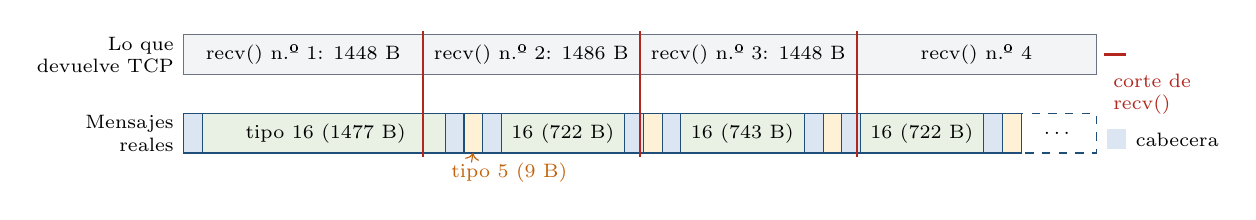
\begin{tikzpicture}[font=\scriptsize, x=0.95cm, y=1cm]
% recv chunks
\foreach \a/\b/\t in {0/3.2/{recv() n.º 1: 1448 B}, 3.2/6.1/{recv() n.º 2: 1486 B}, 6.1/9.0/{recv() n.º 3: 1448 B}, 9.0/12.2/{recv() n.º 4}}{
  \draw[fill=gris, draw=grisT] (\a,1.0) rectangle (\b,1.5); \node at ({(\a+\b)/2},1.25) {\t};}
\node[left, align=right] at (0,1.25) {Lo que\\ devuelve TCP};
% messages
\draw[fill=cHdr, draw=azul] (0,0) rectangle (0.25,0.5);
\draw[fill=cSub, draw=azul] (0.25,0) rectangle (3.5,0.5);  \node at (1.9,0.25) {tipo 16 (1477 B)};
\draw[fill=cHdr, draw=azul] (3.5,0) rectangle (3.75,0.5);
\draw[fill=cArt, draw=azul] (3.75,0) rectangle (4.0,0.5);
\draw[fill=cHdr, draw=azul] (4.0,0) rectangle (4.25,0.5);
\draw[fill=cSub, draw=azul] (4.25,0) rectangle (5.9,0.5); \node at (5.07,0.25) {16 (722 B)};
\draw[fill=cHdr, draw=azul] (5.9,0) rectangle (6.15,0.5);
\draw[fill=cArt, draw=azul] (6.15,0) rectangle (6.4,0.5);
\draw[fill=cHdr, draw=azul] (6.4,0) rectangle (6.65,0.5);
\draw[fill=cSub, draw=azul] (6.65,0) rectangle (8.3,0.5); \node at (7.47,0.25) {16 (743 B)};
\draw[fill=cHdr, draw=azul] (8.3,0) rectangle (8.55,0.5);
\draw[fill=cArt, draw=azul] (8.55,0) rectangle (8.8,0.5);
\draw[fill=cHdr, draw=azul] (8.8,0) rectangle (9.05,0.5);
\draw[fill=cSub, draw=azul] (9.05,0) rectangle (10.7,0.5); \node at (9.87,0.25) {16 (722 B)};
\draw[fill=cHdr, draw=azul] (10.7,0) rectangle (10.95,0.5);
\draw[fill=cArt, draw=azul] (10.95,0) rectangle (11.2,0.5);
\draw[draw=azul, dashed] (11.2,0) rectangle (12.2,0.5); \node at (11.7,0.25) {\dots};
\node[left, align=right] at (0,0.25) {Mensajes\\ reales};
\node[anchor=west] at (3.45,-0.25) {\color{naranja}tipo 5 (9 B)};
\draw[->, naranja] (3.85,-0.12) -- (3.87,0);
% cuts
\foreach \x in {3.2,6.1,9.0}{\draw[rojo, thick] (\x,-0.05) -- (\x,1.55);}
\node[rojo, align=left, anchor=west] at (12.3,0.75) {corte de\\ recv()};
\draw[rojo,thick] (12.3,1.25)--(12.6,1.25);
\fill[cHdr] (12.35,0.05) rectangle (12.6,0.3); \node[anchor=west] at (12.6,0.17) {cabecera};
\end{tikzpicture}
\caption{Los cortes de \code{recv()} (en rojo) no coinciden con los límites de los mensajes. El buffer guarda el trozo que sobra de cada \code{recv()} y lo completa con el siguiente. Las longitudes son las registradas con URSim 5.25.}\label{fig:buffer}
\end{figure}

\vspace{-6pt}
\textbf{Decisiones del buffer.} (i) La longitud se lee \emph{sin consumirla} (\code{unpack\_from}) y solo se borra del buffer cuando el mensaje está completo; el sobrante se queda para la siguiente vuelta. (ii) Una longitud menor que la cabecera o mayor que 64\,kB solo puede significar que el flujo está desalineado. En ese caso no se intenta resincronizar: se lanza \code{ValueError}, el lector cierra la conexión y abre una nueva, que siempre empieza en un límite de mensaje. (iii) Si \code{recv()} devuelve 0 bytes, el robot ha cerrado la conexión, y se trata como tal. (iv) En tiempo real la longitud tampoco es una constante: se lee de cada paquete, de modo que el mismo código funciona con versiones que envían 1140 o 1220 bytes.

\textbf{Verificación ejecutando el código.} Se alimentó \code{extraer\_mensajes} con un flujo de 402 mensajes (con las longitudes de URSim) troceado de 200 formas aleatorias distintas (trozos de 1 a 3000 bytes) y también byte a byte. En todos los casos se obtuvieron los 402 mensajes idénticos y el buffer quedó vacío. Si el flujo empieza 3 bytes desplazado, la primera longitud leída es 873\,725\,952 y la validación lo detecta de inmediato.

\section{Decodificación de los mensajes}

\textbf{Interfaz primaria (30001).} Cada mensaje cortado se identifica por su tipo (byte 4). Del tipo 16 (\emph{Robot State}) se recorren los subpaquetes con \code{offset += longitud\_sub}, sin suponer ningún orden. El tipo 20 (\emph{Robot Message}) solo se decodifica cuando \code{robotMessageType = 6} (código de error). Cualquier otro tipo se ignora: su longitud ya ha permitido saltarlo.

\begin{figure}[h]
\centering
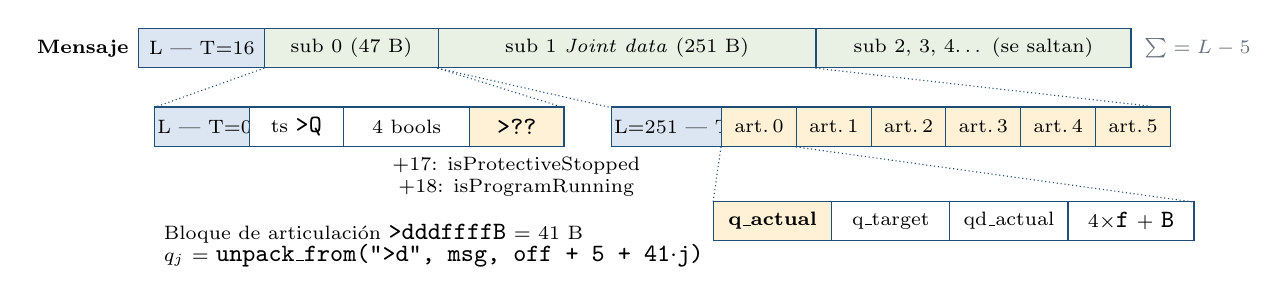
\begin{tikzpicture}[font=\scriptsize, x=1cm, y=1cm]
\tikzset{b/.style={draw=azul, minimum height=5mm, inner sep=1pt, anchor=south west}}
% nivel 1
\node[left] at (0,0.25) {\bfseries Mensaje};
\node[b, fill=cHdr, minimum width=1.6cm] at (0,0) {L | T=16};
\node[b, fill=cSub, minimum width=2.2cm] at (1.6,0) {sub 0 (47 B)};
\node[b, fill=cSub, minimum width=4.8cm] at (3.8,0) {sub 1 \emph{Joint data} (251 B)};
\node[b, fill=cSub, minimum width=4.0cm] at (8.6,0) {sub 2, 3, 4\dots\ (se saltan)};
\node[anchor=west, grisT] at (12.65,0.25) {$\sum = L-5$};
% nivel 2: sub0
\node[b, fill=cHdr, minimum width=1.2cm] at (0.2,-1.0) {L | T=0};
\node[b, fill=white, minimum width=1.2cm] at (1.4,-1.0) {ts \code{>Q}};
\node[b, fill=white, minimum width=1.6cm] at (2.6,-1.0) {4 bools};
\node[b, fill=cArt, minimum width=1.2cm, align=center] at (4.2,-1.0) {\code{>??}};
\node[below, align=center] at (4.8,-1.0) {+17: isProtectiveStopped\\ +18: isProgramRunning};
\draw[densely dotted, azul] (1.6,0) -- (0.2,-0.5); \draw[densely dotted, azul] (3.8,0) -- (5.4,-0.5);
% nivel 2: sub1
\node[b, fill=cHdr, minimum width=1.4cm] at (6.0,-1.0) {L=251 | T=1};
\foreach \j in {0,...,5}{\node[b, fill=cArt, minimum width=0.95cm] at ({7.4+0.95*\j},-1.0) {art.\,\j};}
\draw[densely dotted, azul] (3.8,0) -- (6.0,-0.5); \draw[densely dotted, azul] (8.6,0) -- (13.0,-0.5);
% nivel 3: articulación
\node[b, fill=cArt, minimum width=1.5cm] at (7.3,-2.2) {\bfseries q\_actual};
\node[b, fill=white, minimum width=1.5cm] at (8.8,-2.2) {q\_target};
\node[b, fill=white, minimum width=1.5cm] at (10.3,-2.2) {qd\_actual};
\node[b, fill=white, minimum width=1.6cm] at (11.8,-2.2) {4$\times$\code{f} + \code{B}};
\draw[densely dotted, azul] (7.4,-1.0) -- (7.3,-1.7); \draw[densely dotted, azul] (8.35,-1.0) -- (13.4,-1.7);
\node[anchor=west, align=left] at (0.2,-2.25) {Bloque de articulación \code{>dddffffB} = 41 B\\ $q_j$ = \code{unpack\_from(">d", msg, off + 5 + 41$\cdot$j)}};
\end{tikzpicture}
\caption{Anidamiento mensaje $\rightarrow$ subpaquete $\rightarrow$ articulación en la interfaz primaria, con los campos que lee el programa.}\label{fig:anidado}
\end{figure}

\vspace{-8pt}
\begin{lstlisting}[firstnumber=31]
offset, fin = 5, min(longitud, len(mensaje))
while offset + 5 <= fin:
    longitud_sub, tipo_sub = struct.unpack_from(">iB", mensaje, offset)
    if longitud_sub < 5 or offset + longitud_sub > fin:      # se sale del mensaje: corrupto
        raise ValueError(f"Subpaquete tipo {tipo_sub} con longitud inválida {longitud_sub}")
    if tipo_sub == 0:   ...  # isProtectiveStopped, isProgramRunning en offset+17
    elif tipo_sub == 1: q = [struct.unpack_from(">d", mensaje, offset + 5 + 41*i)[0] for i in range(6)]
    offset += longitud_sub                                   # saltar al siguiente subpaquete
\end{lstlisting}

\textbf{Interfaz de tiempo real (30003).} Hay un único tipo de paquete con los campos en posiciones fijas, así que basta con cortar el paquete y saltar al desplazamiento de cada campo (tabla~\ref{tab:rt}). Los campos de estado solo se leen si el paquete es lo bastante largo; con versiones antiguas quedan a \code{None} en lugar de leer bytes ajenos.

\begin{table}[h]
\centering\small
\caption{Campos de tiempo real usados (hoja \emph{Client Interfaces}, SW 5.x; desplazamiento $=4+8\cdot(\text{índice}-1)$).}\label{tab:rt}
\begin{tabular}{@{}r l l l@{}}
\toprule
Byte & Campo & Formato & Uso en el programa \\ \midrule
0 & Message size & \code{>i} & delimitar el paquete en el buffer (1220 B en URSim 5.25)\\
4 & Time & \code{>d} & reloj del controlador (\code{rx.py} mide con él la tasa real)\\
252 & q actual & \code{>6d} & ángulos de las 6 articulaciones\\
812 & Safety mode & \code{>d} & 3 = parada de protección; 5--9 se tratan como error\\
1052 & Program state & \code{>d} & 2 = programa en ejecución (equivale a \code{isProgramRunning})\\ \bottomrule
\end{tabular}
\end{table}

\section{El estado compartido y el \texttt{Lock}}

Cada robot tiene un diccionario \code{Robot\_state} (\code{q}, \code{isProgramRunning}, \code{isProtectiveStopped}, \code{error}, \code{socket}) y su propio \code{threading.Lock}. El criterio es que \textbf{el lock solo protege copias}. El lector decodifica \emph{fuera} del lock y solo lo toma para asignar los valores ya calculados. Quien consume (el bucle de dibujo, \code{guardar\_posicion} o \code{esperar\_movimiento}) lo toma para copiar (\code{q[:]}) y lo suelta antes de usar los datos. Así las secciones críticas duran microsegundos y el lector de 500\,Hz nunca espera a PyBullet.

\begin{lstlisting}[numbers=none]
# Hilo lector (tiempo_real.py): un único bloque por paquete -> los cuatro campos son coherentes
with lock:
    Robot_state["q"] = list(q);  Robot_state["isProgramRunning"] = program_running
    Robot_state["isProtectiveStopped"] = protective_stopped;  Robot_state["error"] = error
# Hilo principal (multi_robot.py): copiar bajo el lock y dibujar fuera de él
with r["lock"]:
    q = r["Robot_state"]["q"][:]
sim.move_robot(r["id"], q)
\end{lstlisting}

Un lock \emph{por robot}, y no uno global, evita que un robot lento o desconectado retenga a los demás. \code{q} se sustituye por una lista nueva en vez de modificarse elemento a elemento, de modo que ni siquiera un lector sin lock vería una lista a medias. El lock sigue siendo necesario para que \code{q} y los indicadores de estado que se leen juntos procedan del mismo mensaje. Esto se cuantifica en la pregunta~8.

\section{Envío de órdenes (enseñar y reproducir)}

\code{enviar\_movimiento()} valida que haya 6 ángulos finitos dentro de $\pm2\pi$ (para no enviar grados por error), limita $v$ y $a$ a 0,3\,rad/s y 0,5\,rad/s$^2$ y envía \code{def mover(): movej([...], a, v) end}. \code{esperar\_movimiento()} deduce el cumplimiento del estado publicado: espera a que \code{isProgramRunning} pase a verdadero (si no ocurre en 2\,s, la orden se ha rechazado), vigila errores y paradas de protección mientras dura el movimiento, y al terminar exige que la desviación sea menor de 0,01\,rad en cada articulación. La serie se ejecuta punto a punto en un hilo aparte, lo que permite cancelarla (\code{stopj}) y reanudarla desde el punto que falló. Los puntos se guardan en \code{config/puntos.json}.

%================================ PREGUNTAS ================================
\section{Respuestas a las preguntas del apartado 12}

Para las preguntas 1 y 7 el código se ejecutó contra un emulador local de las interfaces 30001 y 30003 que reproduce las longitudes registradas con URSim 5.25 (722, 743, 1477 y 9\,B en la primaria y 1220\,B en tiempo real), a 10\,Hz y 500\,Hz respectivamente. El lector es el \code{buffer\_ur.py} entregado, con un contador del tamaño de cada \code{recv()}. Cada escenario duró 60\,s.

\preg{1}{¿Coincide siempre lo que devuelve \code{recv()} con la longitud de un mensaje?}\label{sec:p1}
\textbf{No.} En la primaria, el robot escribe el mensaje de estado (722\,B) y justo después el de tipo 5 (9\,B), así que el caso habitual es un \code{recv()} de 731\,B con \emph{dos} mensajes dentro. El primer mensaje de estado (1477\,B) es mayor que un segmento Ethernet (MSS $\approx$ 1448\,B) y llega partido en 1448 + 38\,B, es decir, como un mensaje incompleto. En tiempo real, el 99,8\,\% de los \code{recv()} devuelve justo 1220\,B, pero aparecen 2440, 3660 y 4096\,B. Este último caso es el peligroso: 4096 = 3 × 1220 + 436, o sea tres mensajes y un trozo del cuarto. Si el consumidor se retrasa (lo emulamos con una pausa de 20\,ms entre lecturas), el 97\,\% de las llamadas devuelve 4096\,B y en el 99,6\,\% queda un trozo en el buffer.

\begin{table}[h]
\centering\small
\caption{Bytes por \code{recv(4096)} durante 60\,s (emulador local con las longitudes de URSim 5.25).}\label{tab:recv}
\footnotesize
\begin{tabularx}{\linewidth}{@{}l r r X r@{}}
\toprule
Escenario & \code{recv()} & Mensajes & Tamaños devueltos más frecuentes (B) & Con resto \\ \midrule
Primaria (30001) & 603 & 1205 & 731 (×601), 1486, 52 — 2 mensajes por \code{recv} & 0 \\
Primaria, segmentos Ethernet & 604 & 1205 & 731 (×601), \textbf{1448 + 38} (mensaje de 1477 partido) & 1 \\
Tiempo real (30003) & 29\,942 & 30\,001 & 1220 (×29\,890), 2440 (×42), 3660 (×6), \textbf{4096} (×2) & 2 \\
Tiempo real, consumidor lento & 2973 & 9825 & \textbf{4096} (×2881), 2048 (×90) — 3 o 4 mensajes por \code{recv} & 2962 \\ \bottomrule
\end{tabularx}
\end{table}

\vspace{-4pt}
\emph{Consecuencia:} el código no puede suponer \emph{ninguna} relación entre \code{recv()} y los mensajes. Por eso acumula en un buffer, corta por longitud, conserva el sobrante y procesa en un bucle todos los mensajes completos de cada \code{recv()} (sección~2). La captura con URSim (\code{docs/evidencias/salida\_primaria.txt}) confirma que las longitudes son variables: 1477, 743, 722, 881, 181, 57, 55, 52, 24 y 9\,B.

\preg{2}{¿Por qué el mensaje y cada subpaquete empiezan con su longitud? ¿Qué hacer con un subpaquete no documentado?}
Por dos motivos. Primero, \emph{delimitar}: TCP no conserva los límites de los mensajes, así que la longitud es la única forma de saber dónde acaba uno y empieza el siguiente. Segundo, \emph{extensibilidad}: con la longitud se puede saltar un bloque sin entender lo que contiene (\code{siguiente = inicio + longitud}). UR puede añadir subpaquetes o alargar los existentes en versiones nuevas sin romper a los clientes antiguos. Un subpaquete de tipo desconocido simplemente se salta; así lo hace nuestro bucle, que solo actúa sobre los tipos 0 y 1. Lo único que se comprueba es que su longitud no se salga del mensaje: si se sale, el mensaje se descarta como corrupto.

\preg{3}{¿Qué valores salen si se decodifica \code{q\_actual} sin indicar big-endian?}
El robot envía los números en orden de red (big-endian, el byte más significativo primero) y un PC x86 es little-endian. Sin \code{>}, \code{struct} lee los 8 bytes en orden inverso y los interpreta como otro número completamente distinto. Signo, exponente y mantisa salen de bytes que no les corresponden:

\begin{center}\small
\begin{tabular}{@{}l l l l@{}}
\toprule
$q$ enviado (rad) & 8 bytes en el cable (\code{>d}) & Leído con \code{<d} & Leído con \code{>d}\\ \midrule
$-1{,}6007$ (base, punto 10) & \code{bf f9 9c 77 9a 6b 50 b1} & $-3{,}72\times10^{-71}$ & $-1{,}6007$ \\
$1{,}5708$ ($\pi/2$) & \code{3f f9 21 ff 2e 48 e8 a7} & $-1{,}93\times10^{-116}$ & $1{,}5708$ \\
$3{,}14159$ & \code{40 09 21 f9 f0 1b 86 6e} & $2{,}56\times10^{224}$ & $3{,}14159$ \\
$0{,}0$ & \code{00 00 00 00 00 00 00 00} & $0{,}0$ & $0{,}0$ \\ \bottomrule
\end{tabular}
\end{center}

Salen valores casi nulos o astronómicos (del orden de $10^{\pm300}$). Hay un caso traicionero: con el robot en la postura cero todos los bytes son \code{00} y el error no se nota hasta que se mueve. La longitud también se corrompe: 1220 (\code{00 00 04 c4}) leído con \code{<i} da $-1\,006\,370\,816$. Nuestra validación de longitud cortaría la conexión de inmediato.

\preg{4}{Primaria frente a tiempo real. ¿Cuál para un panel de supervisión? ¿Y para registrar un movimiento rápido?}
La \textbf{primaria} (10\,Hz, mensajes variables con subpaquetes) es extensible y además de las posiciones trae información de supervisión: modo del robot, paradas de protección, errores (tipo 20), versión y excepciones de programa. La de \textbf{tiempo real} (500\,Hz, paquete fijo) es sencilla y rápida de decodificar por desplazamientos, y su resolución temporal es 50 veces mayor, pero no trae mensajes de evento y su formato depende de la versión. Para un \emph{panel de supervisión} elegiríamos la primaria, preferiblemente por el puerto de solo lectura 30011: 10\,Hz sobra para el ojo humano y lo importante son los errores y estados. Para \emph{registrar la trayectoria de un movimiento rápido} elegiríamos la de tiempo real: a 10\,Hz, un eje a 3\,rad/s recorre 0,3\,rad entre dos muestras, mientras que a 500\,Hz solo recorre 6\,mrad.

\preg{5}{¿Por qué en NAT no se puede conectar a URSim desde el PC y en modo puente sí? ¿Quién ve la MAC de la VM?}
En NAT, VirtualBox coloca la VM en una red privada interna (10.0.2.x) detrás de un router virtual. Las conexiones \emph{salientes} de la VM se traducen a la IP del PC, pero nadie puede iniciar una conexión \emph{entrante} hacia el puerto 30001 de la VM sin una regla de reenvío de puertos: la IP de la VM no es alcanzable desde fuera. En modo puente, la VM se conecta directamente a la red física con su propia MAC y obtiene una IP de la misma subred (10.172.18.x en el aula), igual que cualquier otro equipo. La MAC de la VM la ven los equipos del mismo dominio de difusión: el switch, que la aprende en su tabla, el PC anfitrión y los demás equipos de la LAN, en sus tablas ARP. No la ven los equipos que están detrás de un router, porque el router reescribe las cabeceras Ethernet en cada salto.

\preg{6}{¿Qué hace el programa al desconectar el cable 5\,s? ¿Qué hace TCP con los datos?}
\emph{TCP:} un corte físico no cierra la conexión, porque no se envía ni FIN ni RST. El robot sigue escribiendo en su buffer de envío y retransmite los segmentos sin ACK con un \emph{timeout} exponencial. Al reconectar el cable, si la conexión sigue viva, entrega los datos pendientes en orden y sin pérdidas. Llegan de golpe y \emph{atrasados}, y si el buffer del robot se ha llenado, este puede dejar de escribir o cerrar la conexión. \emph{Nuestro programa:} sin datos, el \emph{timeout} de recepción salta (1\,s en tiempo real, 2\,s en la primaria) y lanza \code{TimeoutError}. El lector lo captura, marca el socket como \code{None}, cierra y reintenta cada segundo (\code{"Conexión perdida: TimeoutError('timed out'). Reconectando..."}, en las evidencias). El robot dibujado se queda en la última postura conocida y, en el multi-robot, los demás robots siguen moviéndose. Al volver la red, se abre una conexión \emph{nueva} que empieza alineada y con datos frescos, sin la cola atrasada. Si había una serie en ejecución, se detiene por falta de conexión y se reanuda con \code{c}. La figura~\ref{fig:evid} muestra este comportamiento con URSim.

\begin{figure}[h]
\centering
\begin{minipage}[t]{0.47\linewidth}
\begin{lstlisting}[numbers=none,language={},basicstyle=\ttfamily\scriptsize,backgroundcolor=\color{gris}]
Conectado a 192.168.1.140:30001
Recibido mensaje tipo 20 con longitud 55
Recibido mensaje tipo 20 con longitud 24
Recibido mensaje tipo 24 con longitud 181
Recibido mensaje tipo 23 con longitud 881
Recibido mensaje tipo 16 con longitud 1477
Estados de las articulaciones: [ -91.71
  -98.96 -126.22 -46.29  91.39  -1.78]
Recibido mensaje tipo 5 con longitud 9
Recibido mensaje tipo 16 con longitud 743
\end{lstlisting}
\end{minipage}\hfill
\begin{minipage}[t]{0.51\linewidth}
\begin{lstlisting}[numbers=none,language={},basicstyle=\ttfamily\scriptsize,backgroundcolor=\color{gris}]
Tasa de recepcion: 377.00 paquetes/s
Tasa de recepcion: 371.00 paquetes/s
Tasa de recepcion: 308.00 paquetes/s
Conexion perdida: TimeoutError('timed out').
  Reconectando...
Servidor 192.168.1.140:30003 no disponible
  (intento 1): timed out. Reintentando en 1.0 s...
Servidor 192.168.1.140:30003 no disponible
  (intento 2): timed out. Reintentando en 1.0 s...
\end{lstlisting}
\end{minipage}
\caption{Capturas de consola con URSim (\code{docs/evidencias/}). Izquierda: \code{primaria.py} en modo de depuración, con mensajes de tipos y longitudes variables. Derecha: \code{tiempo\_real.py} al apagar URSim: \emph{timeout}, reconexión cada segundo y sin bloqueo.}\label{fig:evid}
\end{figure}


\preg{7}{(N) Retraso entre URSim y el robot simulado con cada interfaz. ¿De qué depende?}
El retraso es la suma de: (a) el \emph{periodo de muestreo}, de 0 a 100\,ms en la primaria y de 0 a 2\,ms en tiempo real; (b) la red y la pila TCP, por debajo de 1\,ms en una LAN; (c) el bucle de dibujo a 30\,Hz, de 0 a 33\,ms; y (d) el refresco de pantalla. Estimado: unos 50--130\,ms con la primaria frente a unos 20--40\,ms con tiempo real. La primaria va visiblemente detrás. El factor crítico es que el \textbf{consumidor siga el ritmo del productor}. En la prueba con el consumidor lento (tabla~\ref{tab:recv}), los datos procesados llegaban cada vez más viejos: 1,3\,s de retraso al cabo de 1\,s, 7,4\,s a los 10\,s y 13,5\,s a los 19\,s, porque la cola de TCP no deja de crecer. Con lectura continua, el retraso se mantuvo en torno a 1\,ms. Por eso la recepción va en un hilo que no dibuja. Con URSim medimos entre 245 y 377 paquetes/s mientras PyBullet dibujaba, y unos 450/s con \code{rx.py}, que compara el reloj del robot con el del PC para separar lo que el simulador envía de lo que nuestra aplicación consume.

\preg{8}{(N) ¿Qué pasaría si el bucle de PyBullet leyera el estado sin \code{Lock} mientras otro hilo lo escribe?}
Leería un estado \emph{inconsistente}: mezcla de dos mensajes distintos. Lo comprobamos con un hilo que imita al lector (300\,000 escrituras) y otro que imita a \code{esperar\_movimiento}, forzando cambios de hilo frecuentes (\code{sys.setswitchinterval(1e-6)}) para simular carga:

\begin{center}\small
\begin{tabular}{@{}l c c@{}}
\toprule
Forma de compartir el estado & \shortstack{$q$ con ángulos\\de dos mensajes} & \shortstack{$q$ y \code{isProgramRunning}\\de mensajes distintos} \\ \midrule
Sin lock, $q$ modificado elemento a elemento & 57,5\,\% de las lecturas & 5,1\,\% \\
Lock por campo (secciones separadas) & 0\,\% & 64,5\,\% \\
\textbf{Un lock por mensaje} (como en \code{tiempo\_real.py}) & \textbf{0\,\%} & \textbf{0\,\%} \\ \bottomrule
\end{tabular}
\end{center}

En el visualizador, el efecto sería un parpadeo o una postura que nunca existió. El riesgo real está en el control: si \code{esperar\_movimiento} leyera \code{isProgramRunning = False} del mensaje nuevo junto con un $q$ del anterior, daría por terminado o por fallido un movimiento que no lo está. El GIL de CPython hace atómica una asignación individual, pero \emph{no} un grupo de lecturas o escrituras. El lock garantiza esa atomicidad de grupo. Los porcentajes están inflados por la prueba de estrés: a 500\,Hz la ventana es de microsegundos y el fallo es raro, pero precisamente por eso es difícil de depurar. \emph{Mejora pendiente:} en \code{primaria.py} los subpaquetes 0 y 1 se publican en dos bloques \code{with lock} separados, el caso de la fila central. Acumular ambos y publicarlos en un único bloque por mensaje eliminaría esa ventana.

\preg{9}{(S) ¿Por qué no basta con haber enviado un \code{movej}? ¿Qué información del robot se usa para confirmarlo?}
\code{sendall()} solo garantiza que los bytes han salido de nuestro buffer, y el ACK de TCP, que han llegado a la pila del controlador. Ninguno dice si el programa se ha aceptado, ni si se ha ejecutado o completado. El robot puede rechazarlo (no está en modo remoto, la conexión es de solo lectura, error C210), abortarlo por una parada de protección o detenerlo por otro programa que llegue después. Además, el controlador no envía ninguna respuesta a la orden. Confirmamos con el estado que el robot sigue publicando: \code{isProgramRunning} (subpaquete 0, o \code{program\_state} = 2 en tiempo real) pasa a verdadero en menos de 2\,s y vuelve a falso, y durante ese tiempo no hay \code{isProtectiveStopped} (o \code{safety\_mode} = 3) ni mensajes de error tipo 20 / subtipo 6. Al final, $|q_{\text{actual}}-q_{\text{objetivo}}|<0{,}01$\,rad en las seis articulaciones. Si se supera el tiempo esperado se envía \code{stopj}.

\preg{10}{(S) Riesgo de que cualquier equipo pueda enviar programas al 30001 y dos medidas.}
Cualquier equipo de la red de planta, o un atacante que haya entrado en ella, podría mover un robot con personas cerca, cambiar programas o velocidades, provocar paradas (denegación de servicio) o leer información del proceso. No hay autenticación ni cifrado: el URScript viaja en texto plano. \emph{Medida en el robot:} en PolyScope, \emph{Ajustes} $\rightarrow$ \emph{Seguridad} $\rightarrow$ \emph{Servicios}, deshabilitar los puertos que no se usen o dejarlos en solo lectura (los visualizadores, por 30011/30012), y mantener el robot en modo \emph{Local}, pasando a \emph{Remoto} solo cuando se autorice el control externo. \emph{Medida en la red:} segmentar la célula en una VLAN propia, siguiendo el modelo de zonas y conductos de IEC 62443, detrás de un cortafuegos con lista blanca que solo permita llegar al 30001 desde la IP del PC de control. Los demás equipos acceden a los datos a través de una pasarela de solo lectura.

\end{document}
